\section{Optimizing Pointwise Convolution}
\label{sec:pwconv}
In this section, we demonstrate the workflow of our dynamic blocking strategy as shown in Figure \ref{fig:pwflow} and Algorithm \ref{algo:pwalgo}. 
The whole workflow consists of two stages. 

In the first stage, our approach operates in a top-down fashion. 
We use a 4-level hierarchical partitioning method to decompose the output into four levels of tiles, including SM level tiles, block level tiles, warp level tiles and thread level tiles. 
There are two main considerations when decomposing the output. First, how tiles are arranged in its upper level tile, and second, the height and width of each tile with the specified layout.

In the second stage, we calculate the exact height and width of thread level tiles. Given the number of output elements in each tile and hardware resources constraints, we iterate over all possible layout combinations of each level and choose the combination that maxmize the aritemetic intensity of a thread.

Now we give a detailed description of how each stage works.
\subsection{4-Level Hierarchical Partitioning}
In order to make it easier to understand the workflow of this stage, we first describe two important constant parameters and how we determine their values.

The first parameter is the number of warps in a thread block, denoted as $Warp_{num}$.
In order to determin the warp number, we need to consider: (1) small warp number will decrease the opportunity to hide the memory access latency at the warp level;
(2) large warp number will dcrease the number of thread blocks and may lead to SM underutilization.
Baed on both considerations, we decide to set $Warp_{num}=4$.
In our experiments, this value is good enough to provide a satisfied performance.

%this may not be important as i think
%The second parameter is the number of thread blocks that can run concurrently in an SM, denoted as $Block_{num}$.
%We use three values, 2, 4 and 6, for this parameter, denoted as $Block_{Num}=\{2, 4, 6\}$. 
%There are two reasons for these choices: 
%(1) when $Block_{num}=1$, there are only 4 warps in an SM. 
%As each thread can use up to 256 registers, a thread block can use at most $4*32*256=32768$ registers, which is only 50\% of registers of an SM.
%To avoid wasting hardware resources, we set $Block_{num}>1$; 
%(2) when $Block_{num}>6$, each thread can use at most 70 registers and thus requires careful optimization on register usage to avoid register spills.
%In our experiments, $Block_{num}=\{2, 4\}$ are the most commonly used values.

Now we demonstrate the workflow of 4-level hierarchical partitioning.
In our design, we can either distribute filter channels or input channels across threads. 
Therefore, we have two choices for the output layout and the corresponding logical views are shown in Figure \ref{fig:pwworkflow}.
For the output dimension that represents filter, we call it filter dimension, and the other one input dimension.
When partition the output into SM tiles, we always operate on the filter dimension and thus two layouts can share the same partition methods.
We design two partition methods, one divides the filter dimension into halves and the other keeps the filter dimension unchanged.
Once the partition method is decided, we can calculate the width of an SM tile in layout \textbf{\emph{L1}} with $SM_{W}=\{F_N/2,F_N\}$ and the height of an SM tile in layout \textbf{\emph{L2}} with $SM_{H}=\{F_N/2,F_N\}$.
In order to determine the size of the other dimension of an SM tile, we need to know the number of output elements in an SM tile.
When GPU is fully utilized, all $O_{size}$ output elements need to be distributed across all SMs, denoted as $SM_{num}$.
And the number of output elements in each SM tile is $SM_{size}=O_{size}/SM_{num}$.
Therefore, the height of an SM tile in layout \textbf{\emph{L1}} is $SM_{H}=SM_{size}/SM_W$ and the width of an SM tile in layout \textbf{\emph{L2}} is $SM_{W}=SM_{size}/SM_H$.

Now we get the height and width of an SM tile, {\color{red}the next step}is to partition the SM tile into block tiles.
We use the aforementationed partition method to divide the SM tile into block tiles, then the width of the block tile can be calculated as $Block_{W}=\{SM_W/2,SM_W\}$.
As mentioned earlier, each SM contains $Block_{num}$ thread blocks. 
We first divide each SM tile into $Block_{num}$ block tiles, and the height of a block tile is $Block_{H}=SM_{size}/Block_{num}/Block_{W}$.
To calculate the height of the SM tile, we first assume that each SM tile only contains 2 block tiles and the height of a block tile is $Block_{H}=SM_{size}/2/Block_{W}$.




For each block number, there are two block tile layout, a column of block tiles or a row of block tiles. 
Then the height and width of a block tile can be denoted as $BlockTile_W=\{F_H, \frac{F_H}{2}\}$, $BlockTile_H=\frac{SM_{tile}}{BlockTile_W}$.

After deciding the number of thread blocks and warps, we can calculate the size of a block tile as $B_{tile}=\frac{SM_{tile}}{Num_{block}}$ and warp tile as $W_{tile}=\frac{B_{tile}}{Num_{warp}}$.
The warp tile layout is fixed as a $2\times2$ matrix, and the height and width can be calculated as $WarpTile_H=\frac{BlockTile_H}{2}$ and $WarpTile_W=\frac{BlockTile_W}{2}$.

Now we demonstrate how to distribute input channels among a warp and calculate the exact shape of each tile.
To map input channels to threads, we need to decide how many threads of a warp calculate continous channels of one output element, denoted as $C_{num}$. 
Figure \ref{fig:pwflow} demonstrates that we use 8 threads to calculate 8 channels of one output element at the same time. 
As there are 32 threads in a warp, we have 6 choices for $C_{num}$, which are $C_{num}=\{1,2,4,8,16,32\}$.

For each option of $C_{num}$, we calculate how many filters a warp can process at the same time, denoted as $F_{count}=\frac{32}{C_{num}}$. Then we get the number filters each thread needs to process, denoted as $T_{filter}=\frac{WarpTile_W}{F_{count}}$.
Based on these informantion and hardward constraints, we choose a combination of $Num_{block}$, block tile layout, and $C_{num}$ to maxmize the aritemetic intensity of a therad.
\begin{figure}
	\centering
    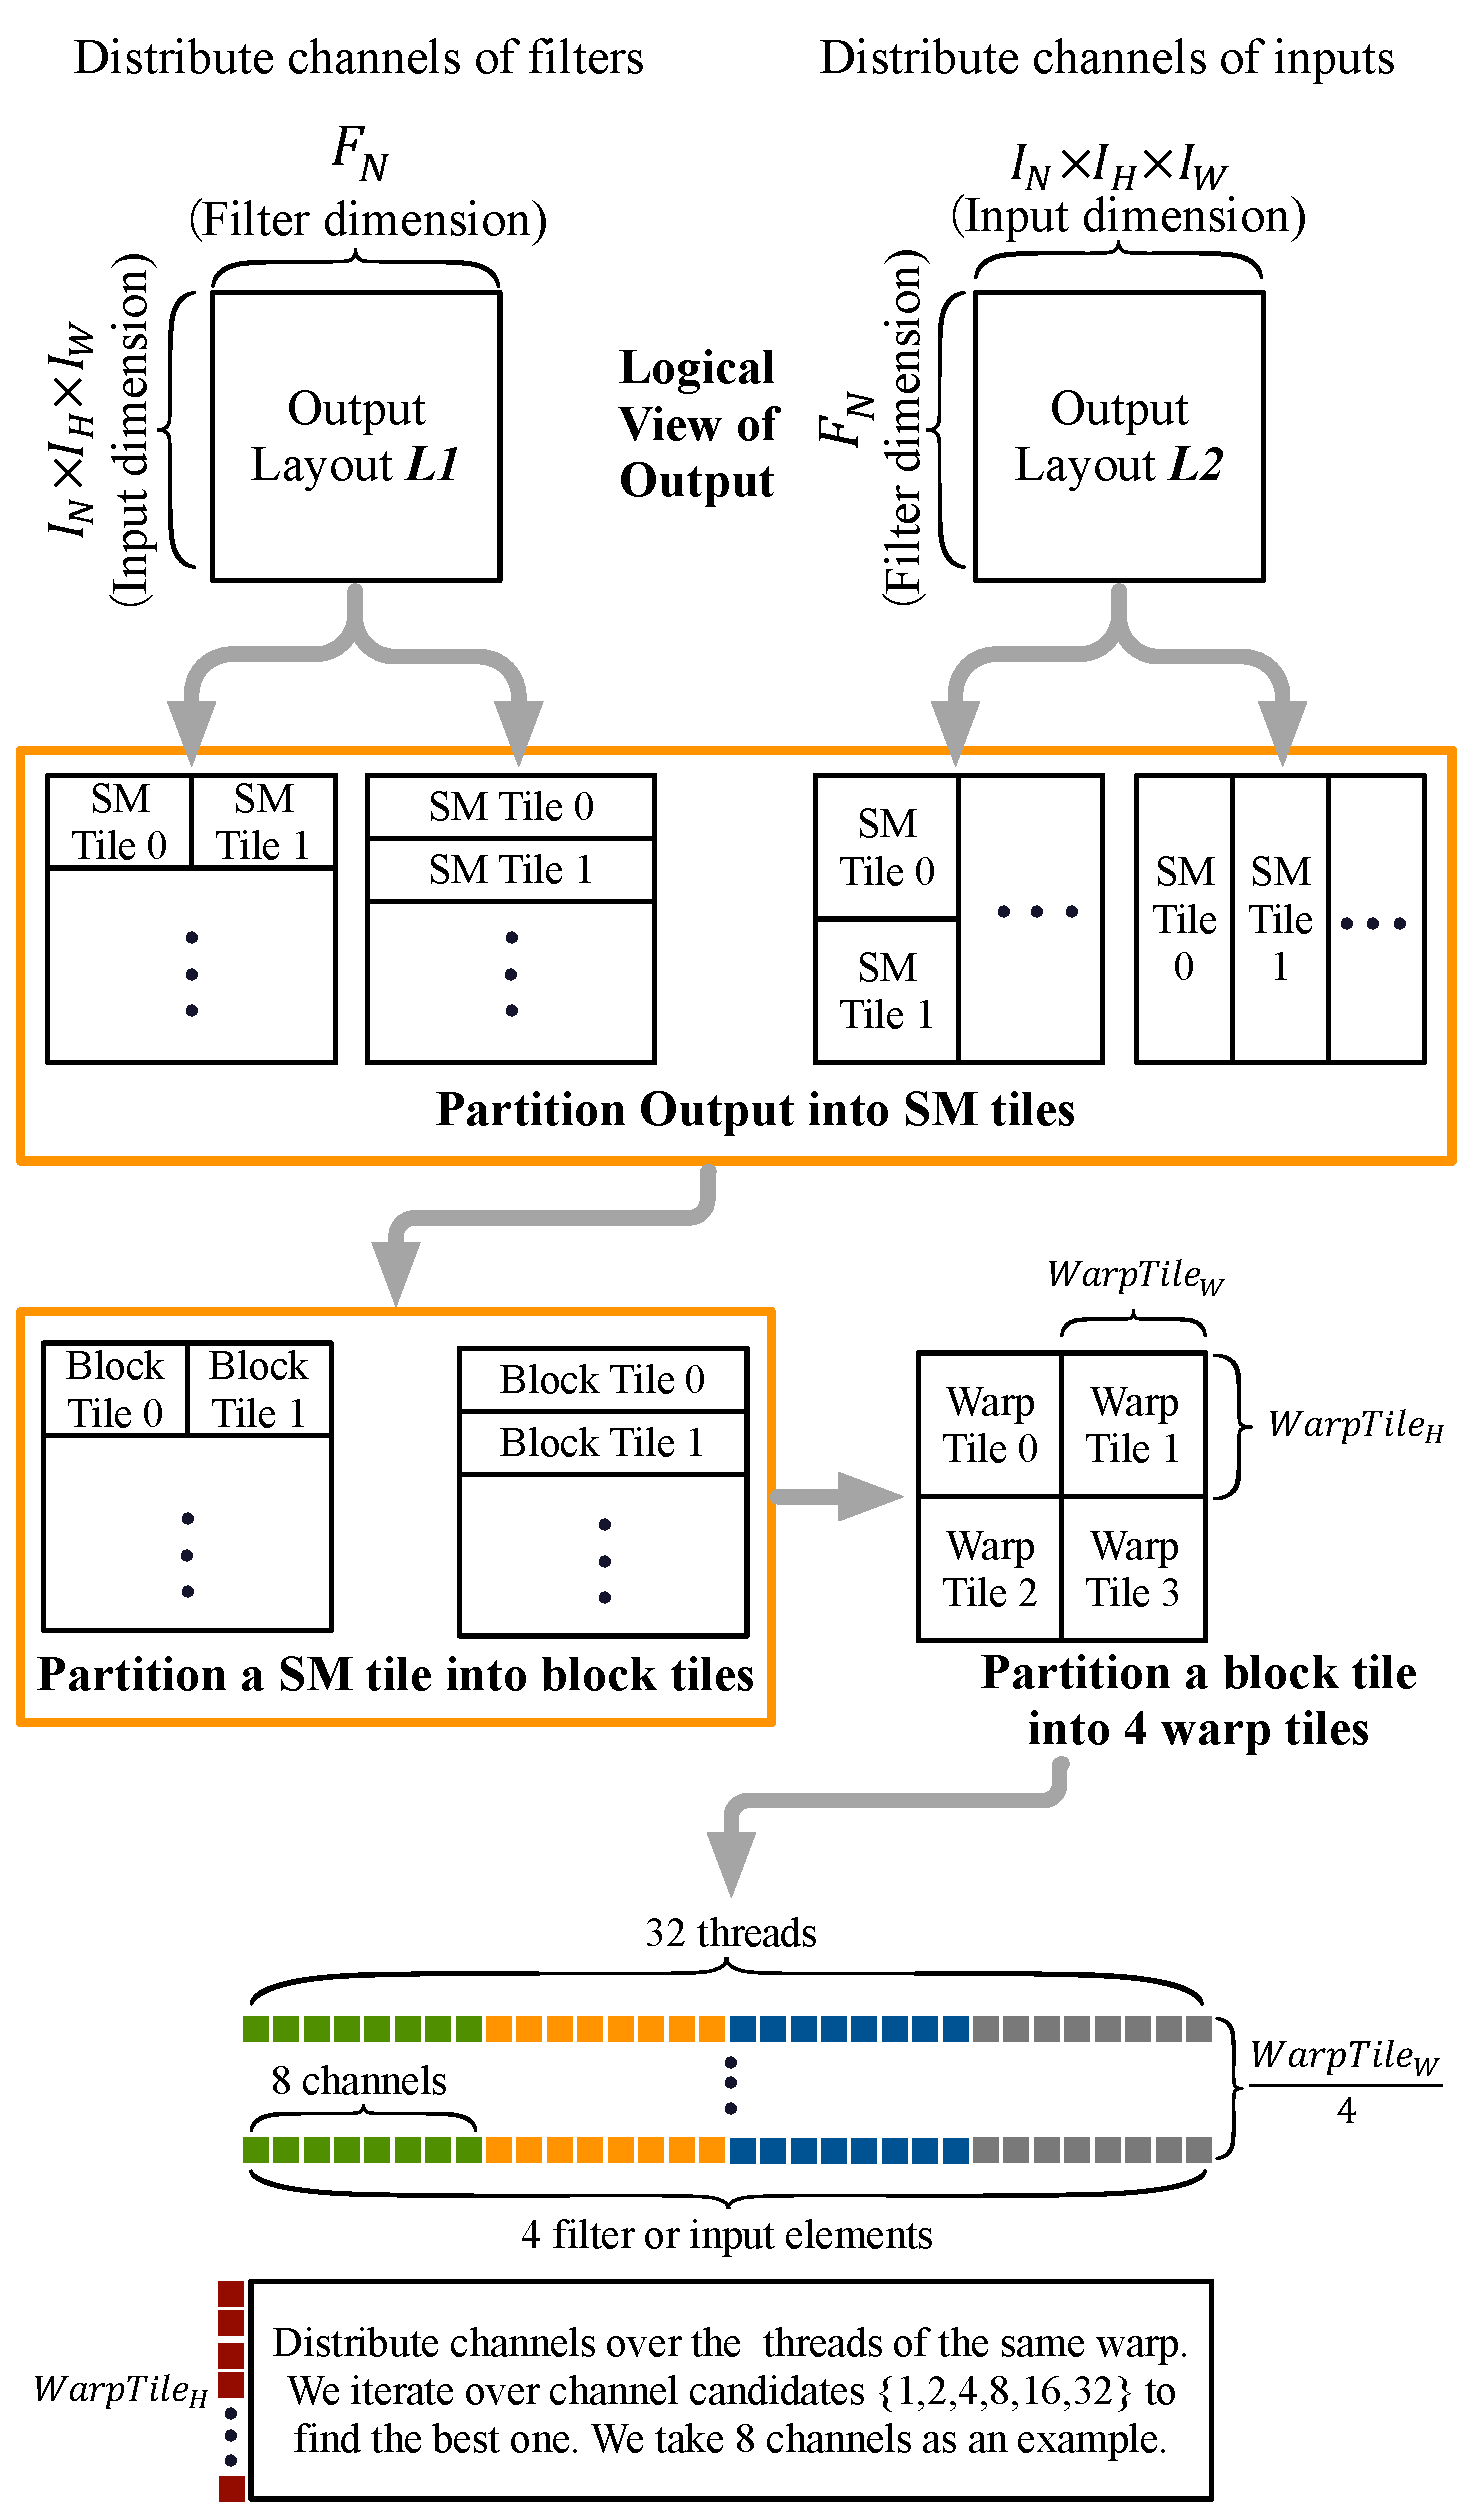
\includegraphics[width=\columnwidth]{./figure/pwworkflow.eps}
    \caption{} \label{fig:pwworkflow}
\end{figure}
\begin{algorithm}[t!]
    \small
        \KwIn{$I$, $F$}
        \KwOut{$O$}
        Calculate how many output elements one SM needs to process if we want to fully utilize GPU, denoted as $O_{sm}$\;
        \tcp{below codes are executed on CPU}
        \tcp{we have two options for block tile number, one SM contains 2 or 4 block tiles}
        \ForEach{block tile number of one SM}{
            Use $BlockTile_{count}$ to denote the number of block tiles resided on one SM\;
            \ForEach{block layout}{
                Calculate the width of a block tile, denoted as $BlockTile_W$\;
                $BlockTile_H = \frac{O_{sm}}{BlockTile_W * BlockTile_{count}}$\;
                \If{$BlockTile_H > 32$}{
                    $niter = BlockTile_H/32$\;
                    $BlockTile_H = 32$\;
                }
                $WarpTile_H=\frac{BlockTile_H}{2}$\;
                $WarpTile_W=\frac{BlockTile_W}{2}$\;
                \tcp{there are 6 choices for channel count, 1,2,4,8,16,32}
                \ForEach{channel count}{
                    Use $C_{count}$ to denote how many threads are uesed to calculate channels of the same output element.\;
                    $filter_{num} = \frac{32}{C_{count}}$\;
                    $filter_{num} = \frac{WarpTile_W}{filter_{num}}$\;
                    Calculate registers and shared memory usage under this configuration, and evaluate if the usage not exceeds the limit.\;
                    record the configuration with smallest register usage. 
                }
            }
        }
        \tcp{below codes are executed on GPU}
        All threads in a thread block cooperate to load the needed input and filter into shared memory\;
        $\_\_syncthreads()$\;
        \For{$iter \gets 0$ \KwTo $I_C$ By $C_{count}$}{
            load next $C_{count}$ channels for input and filter into registers\;
            load current channels of input and filter into registers\;
            calculate output elements\;
            write registers of next channels into shared memory\;
        }
        use segmented parallel reduce to get the final output elements and write the result to global memory\;
        \caption{Pointwise Convolution Optimization}
        \label{algo:pwalgo}
\end{algorithm}